\documentclass[11pt, reqno]{amsart}
\usepackage[sectionbib,numbers]{natbib}
\usepackage{bibunits}
\defaultbibliographystyle{plain}
\defaultbibliography{SplinesBib}
\usepackage{graphicx}
\usepackage{amsmath,amsthm,amssymb}
\usepackage{mathtools}
\usepackage{bm}
\usepackage{fullpage}
\usepackage{enumerate}
\usepackage[margin=2.5cm]{geometry}
\usepackage{hyperref}
\hypersetup{
	colorlinks=true, 
	linkcolor=blue, 
	citecolor=blue, 
	filecolor=blue,
	urlcolor=blue
}
\usepackage{tikz-cd}
\setlength{\marginparwidth}{2cm}
\usepackage{todonotes}
\usepackage{tikz}
\usepackage{blkarray}


\title{Approximation Theory Focus Group - The Fields Institute 2025 - A restriction map and applications to freeness, with emphasis on hyperplane arrangements}
\author{Michael DiPasquale and Nelly Villamizar}
\date{\today}

\newcommand{\RR}{\mathbb{R}}
\newcommand{\R}{\mathbb{R}}
\newcommand{\ZZ}{\mathbb{Z}}
\newcommand{\br}{\mathbf{r}}
\newcommand{\Z}{\mathbb{Z}}
\newcommand{\calJ}{\mathcal{J}}
\newcommand{\calS}{\mathcal{S}}
\newcommand{\calR}{\mathcal{R}}
\newcommand{\A}{\mathcal{A}}
\usepackage[shortlabels]{enumitem}
\newtheorem{theorem}{Theorem}[section]
\newtheorem{lemma}[theorem]{Lemma}
\newtheorem{proposition}[theorem]{Proposition}
\newtheorem{corollary}[theorem]{Corollary}
\newtheorem{conjecture}[theorem]{Conjecture}
\theoremstyle{definition}
\newtheorem{definition}[theorem]{Definition}
\newtheorem{example}[theorem]{Example}
\newtheorem{question}[theorem]{Question}
\theoremstyle{remark}
\newtheorem{remark}[theorem]{Remark}
\numberwithin{equation}{section}

\begin{document}

\maketitle

\section{Setup}

Notation:
\begin{enumerate}
\item $\Sigma$: a pure, hereditary, $n$-dimensional polyhedral fan in $\RR^n$.
\item $\Sigma_i$: $i$-dimesnional cones of $\Sigma$
\item $|\Sigma|=\bigcup_{\sigma\in\Sigma_n}\sigma$.
$\Sigma$ is \textit{complete} if $|\Sigma|=\RR^n$
\item $R$: The polynomial ring $\RR[x_1,\ldots,x_n]$
\item Smoothness distribution or smoothness parameters $\br:\Sigma_{n-1}\to \ZZ_{\ge -1}$.  If $G=(V,E)$ is a graph we will also use $\br$ to denote a map $\br:E\to \ZZ_{\ge -1}$.  We choose this notation so that it matches when $G$ is the \textit{dual graph} of $\Sigma$.
\item $S^\br(\Sigma)$: the $S$-algebra of functions $F:|\Sigma|\to \RR$ that are piecewise polynomial on $\Sigma_n$ and differentiable to order $\br(\tau)$ across the codimension one face $\tau$, for all $\tau\in\Sigma_{n-1}$.
\item $H$: A hyperplane, the zero locus of a linear form $\alpha_H\in R_1$.
\item $\A$: a \textit{central} hyperplane arrangement $\A=\cup_{i=1}^k \mathbb{V}(\alpha_i)$, where $\alpha_i\in R_1$ is a linear form for $i=1,\ldots,k$.
\item $\Sigma^\A$: the complete fan induced by the hyperplane arrangement $\A$, whose maximal cones are the closure (in the Euclidean topology) of the connected components of the complement $\R^n\setminus\A$.
\item $\calR[\Sigma]$: the cellular chain complex (with coefficients in $R$) for $\Sigma$.  The homology is the \textit{Borel-Moore} homology with coefficients in $R$.  This is equivalent to the homology of $B^n\cap\Sigma$ relative to $\partial B^n=\mathbb{S}^n$, where $B^n$ is the unit ball in $\R^n$.
\item $J^{\br}(\tau)$: Here $\tau\in\Sigma_{n-1}$, and the linear span of $\tau$ is defined by the linear form $\alpha_\tau\in R_1$.  By definition, $J^{\br}(\tau)=\langle \alpha_\tau^{\br(\tau)+1}\rangle$.
\item $J^{\br}(\gamma)$: Here $\gamma\in\Sigma_i$, $0\le i\le n-1$.  By definition, $J^{\br}(\gamma)=\sum_{\tau\ni\gamma} J^{\br}(\tau)=\langle \alpha_\tau^{\br(\tau)+1}: \gamma\in\tau\rangle$.
\item $\calJ^{\br}[\Sigma]$:  Abbreviated $\calJ$ if $\br$ and $\Sigma$ are understood.  The sub-complex of $\calR$ with modules $\calJ_n=0$ and $\calJ_i=\bigoplus_{\gamma\in\Sigma_i} J^{\br}(\gamma)$ for $0\le i\le n$.
\item $\calR/\calJ^{\br}[\Sigma]$: Abbreviated $\calR/\calJ$ if $\br$, $\Sigma$ understood.  The quotient of the chain complex $\calR[\Sigma]$ by the subcomplex $\calJ^{\br}[\Sigma]$.
\item $G=(V,E)$: A graph with vertices $V$ and edges $E$
\item $\ell:E\to R$: A map associating each edge of $G$ to a linear form of $R$.
\item $S^{\br}(G,\ell)$ (simply $S^{\br}(G)$  if $\ell$ is understood): the $R$-module of \textit{generalized splines} on the edge-labeled graph $(G,\mathcal{I})$ with map $\mathcal{I}:E\to \{\mbox{ideals of } R\}$ defined by $\mathcal{I}(e)=\langle \ell(e)^{\br(e)+1}\rangle$, as defined in ~\cite{Gilbert-Tymoczko-Viel-2016}.
\end{enumerate}

\begin{remark}
Suppose $\Sigma$ is a pure, hereditary, $n$-dimensional fan in $\R^n$, and $G$ is its dual graph.  That is, $G=(V,E)$ is the graph with a vertex $v_\sigma$ for each $\sigma\in\Sigma_n$ and $v_{\sigma},v_{\sigma'}$ are connected by an edge if and only if $\sigma\cap\sigma'=\tau\in\Sigma_{n=1}$.  By definition each edge $e$ of $G$ corresponds to a codimension one cone $\tau\in\Sigma_{n-1}$.

Let $\br:\Sigma_{n-1}\to \ZZ_{\ge -1}$ be a smoothness distribution.  By a slight abuse of notation we identify $\Sigma_{n-1}$ with $E$, and so also regard $\br$ as a map $\br:E\to\ZZ_{\ge -1}$.  Then $S^{\br}(\Sigma)=S^{\br}(G)$.
\end{remark}

\begin{remark}
It is well-known that the spline module $S^{\br}(\Sigma)$ has a similar structure as the \textit{module of derivations} $D(\A)$ of a hyperplane arrangement (and the module $D(\A,\mathbf{m})$ of multi-derivations, where $\mathbf{m}$ assigns a multiplicity to each hyperplane -- playing the analogous role to $\br$ for splines).  The module of derivations was introduced by Saito (citation needed), while Ziegler showed in~\cite{Ziegler-Multiarrangements-1989} that multi-derivations show up naturally in the study of derivations via restriction.

The study of derivations and multi-derivations is much more developed from an algebraic point of view than is the study of splines.
\end{remark}

\begin{remark}
A difficult and subtle question is to determine when the spline module $S^{\br}(\Sigma)$ is \textit{free}.  When $\Sigma$ is \textit{simplicial}, Schenck shows in~\cite{Spect} that $S^{\br}(\Sigma)$ is free if and only if $H_i(\calR/\calJ[\Sigma])=0$ for $0\le i\le n$.  This criterion can be extended to non-simplicial fans that meet a certain (somewhat technical) hypothesis.  In particular, the criterion holds for the fan induced by a hyperplane arrangement (need notes on this).
\end{remark}

\begin{remark}
Freeness of the spline module turns out to be related to resolving ideals generated by powers of linear forms (sometimes called \textit{power ideals} in the literature).  A first glimpse of this may be seen in~\cite[Lemma~9.12]{AssHom}, where it is shown that, for a complete fan $\Sigma\subseteq \R^3$, $H_2(\calR/\calJ[\Sigma])$ is isomorphic to the syzygy module of the ideal $J^{\br}(\mathbf{0})$ modulo the sum of syzygy modules of the ideals $J^{\br}(\gamma)$ for $\gamma\in \Sigma_1$.
\end{remark}

\section{Saito-Rose determinantal criterion for freeness}

A well-known criterion for the freeness of the module of derivations $D(\A)$ and the module of multi-derivations $D(\A,m)$ is a determinantal criterion known as \textit{Saito's criterion}.  In~\cite{Rose-Module-Bases}, Rose gives an analogous criterion for the freeness of the spline module $S^{\br}(\Delta)$.  (There is an interesting result in~\cite{Samet-Basis-2024} which extends the Saito-Rose criterion to generalized splines on graphs $S^{\br}(G)$ over a factorial domain).

In the following theorem, suppose $F_1,\ldots,F_k$ are splines in $S^{\br}(\Sigma)$.  Write $F_{ij}$ for $(F_j)|_{\sigma_i}$, where $\sigma_1,\ldots,\sigma_n$ is an enumeration of the full-dimensional cones of $\Sigma$.  We write $\begin{bmatrix} F_1 \cdots F_n\end{bmatrix}$ for the $n\times k$ matrix whose entry in row $i$ and column $j$ is $F_{ij}$.  The following theorem is~\cite[Theorem~2.3]{Rose-Module-Bases}, stated in slightly more generality.

\begin{theorem}[{\cite[Theorem~2.3]{Rose-Module-Bases}}]\label{thm:Saito-Rose-determinant}
Suppose $\Sigma\subset\RR^n$ is a pure, hereditary, $n$-dimensional fan with $\ell$ full-dimensional cones.  Let $\br:\Sigma_{n-1}\to \ZZ_{\ge 0}$ be a smoothness distribution.  Then a collection $\{F_1,\ldots,F_\ell\}$ of splines in $S^{\br}(\Sigma)$ is a free basis for $S^{\br}(\Sigma)$ if and only if $\det \begin{bmatrix} F_1 \cdots F_\ell\end{bmatrix}=cQ$ for some non-zero constant $c$, where $Q=\prod_{\tau\in\Sigma_{n-1}} \alpha_\tau^{\br(\tau)+1}$.
\end{theorem}

As an immediate corollary we obtain

\begin{corollary}[{\cite[Corollary~2.4]{Rose-Module-Bases}}]\label{cor:Saito-Rose-simplified}
Let $\Sigma\subset \RR^n$ and $\br$ be as in the statement of Theorem~\ref{thm:Saito-Rose-determinant}.  A collection $\{F_1,\ldots,F_n\}$ of $S$-linearly independent homogeneous elements of $S^{\br}(\Sigma)$ form a basis over $S$ if and only if $\sum_{i=1}^n \deg(F_i)=\sum_{\tau\in\Sigma_{n-1}} (\br(\tau)+1)$.
\end{corollary}


\begin{example}
We illustrate 
	%Here is an example where the restriction map $\pi$ happens to be surjective for all choices of smoothness parameter and hyperplane (this is not usually the case).  For simplicity we will consider a subset of the smoothness parameters where we require cones of the same slope to have the same smoothness parameter.  
	Let $\Sigma$ be the fan in $\RR^2$ with the four cones shown below.  The one-dimensional cones $\tau_1,\tau_2,\tau_3,\tau_4$ are also labeled.
	
	\vspace{10 pt}
	
	\begin{minipage}{.45\textwidth}
		\begin{align*}
			\sigma_1 & =\left\lbrace (x,y)\in\RR^2: x\ge 0, y\ge 0\right\rbrace\\
			\sigma_2 & =\left\lbrace (x,y)\in\RR^2: x\ge 0, y\le 0\right\rbrace\\
			\sigma_3 & =\left\lbrace (x,y)\in\RR^2: x\le 0, y\ge 0\right\rbrace\\
			\sigma_4 & =\left\lbrace (x,y)\in\RR^2: x\le 0, y\le 0\right\rbrace			
		\end{align*}
	\end{minipage}
	\begin{minipage}{.5\textwidth}
		\centering
		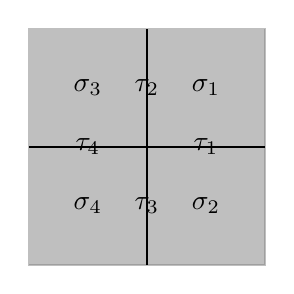
\begin{tikzpicture}[scale=1.5]
			\filldraw[fill=gray, draw=gray, opacity=.5] (-1,-1)--(-1,1)--(1,1)--(1,-1)--cycle;
			
			\draw[thick, black] (-1,0)--(1,0)  (0,-1)--(0,1);
			\node at (.5,.5){$\sigma_1$};
			\node at (-.5,.5){$\sigma_3$};
			\node at (-.5,-.5){$\sigma_4$};
			\node at (.5,-.5){$\sigma_2$};
			\node at (0,.5){$\tau_2$};
			\node at (-.5,0){$\tau_4$};
			\node at (0,-.5){$\tau_3$};
			\node at (.5,0){$\tau_1$};
		\end{tikzpicture}
	\end{minipage}
	
	\vspace{10 pt}
	
	Let us choose smoothness distribution $\br(\tau_2)=\br(\tau_3)=a\in \ZZ_{\ge 0}$ and $\br(\tau_1)=\br(\tau_4)=b\in\ZZ_{\ge 0}$.  Put $R=\RR[x,y]$.  This is one case where we can easily write down generators for $S^{\br}(\Sigma)$.  We have $\alpha_{\tau_2}=\alpha_{\tau_3}=x$ and $\alpha_{\tau_1}=\alpha_{\tau_4}=y$.
	
	We record a spline $F\in S^{\br}(\Sigma)$ as a tuple $(F_{\sigma_1},F_{\sigma_2},F_{\sigma_3},F_{\sigma_4})$ or in transposed form as a column vector.  Put $F_{\sigma_i}=F_i$ for $i=1,2,3,4$.  There are four natural splines: $F_1=(x^{a+1}y^{b+1},0,0,0), F_2=(x^{a+1},x^{a+1},0,0), F_3=(y^{b+1},0,y^{b+1},0),$ and $F_4=(1,1,1,1)$ (check the spline conditions):
	
	\begin{center}
		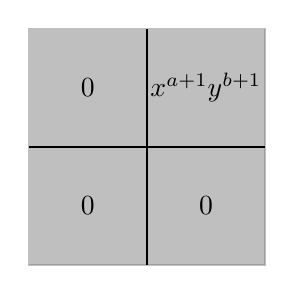
\begin{tikzpicture}[scale=1.5]
		\filldraw[fill=gray, draw=gray, opacity=.5] (-1,-1)--(-1,1)--(1,1)--(1,-1)--cycle;
		
		\draw[thick, black] (-1,0)--(1,0)  (0,-1)--(0,1);
		\node at (.5,.5){$x^{a+1}y^{b+1}$};
		\node at (-.5,.5){$0$};
		\node at (-.5,-.5){$0$};
		\node at (.5,-.5){$0$};
	\end{tikzpicture}
		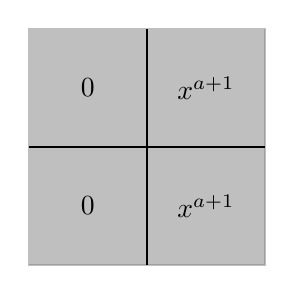
\begin{tikzpicture}[scale=1.5]
			\filldraw[fill=gray, draw=gray, opacity=.5] (-1,-1)--(-1,1)--(1,1)--(1,-1)--cycle;
			
			\draw[thick, black] (-1,0)--(1,0)  (0,-1)--(0,1);
			\node at (.5,.5){$x^{a+1}$};
			\node at (-.5,.5){$0$};
			\node at (-.5,-.5){$0$};
			\node at (.5,-.5){$x^{a+1}$};
		\end{tikzpicture}
		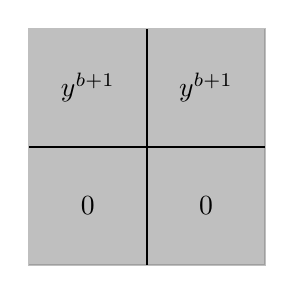
\begin{tikzpicture}[scale=1.5]
			\filldraw[fill=gray, draw=gray, opacity=.5] (-1,-1)--(-1,1)--(1,1)--(1,-1)--cycle;
			
			\draw[thick, black] (-1,0)--(1,0)  (0,-1)--(0,1);
			\node at (.5,.5){$y^{b+1}$};
			\node at (-.5,.5){$y^{b+1}$};
			\node at (-.5,-.5){$0$};
			\node at (.5,-.5){$0$};
		\end{tikzpicture}
				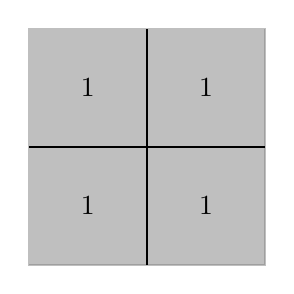
\begin{tikzpicture}[scale=1.5]
			\filldraw[fill=gray, draw=gray, opacity=.5] (-1,-1)--(-1,1)--(1,1)--(1,-1)--cycle;
			
			\draw[thick, black] (-1,0)--(1,0)  (0,-1)--(0,1);
			\node at (.5,.5){$1$};
			\node at (-.5,.5){$1$};
			\node at (-.5,-.5){$1$};
			\node at (.5,-.5){$1$};
		\end{tikzpicture}
	\end{center}
	
	Putting these as column vectors into a matrix we get:
	\begin{equation*}
		\begin{blockarray}{ccccc}
			& F_1 & F_2 & F_3 & F_4 \\
			\begin{block}{c[cccc]}
				\sigma_1 & x^{a+1}y^{b+1} & x^{a+1} & y^{b+1} & 1 \\ 
				\sigma_2 & 0 & x^{a+1} & 0 & 1 \\
				\sigma_3 & 0 & 0 & y^{b+1} & 1 \\
				\sigma_4 & 0 & 0 & 0 & 1 \\
			\end{block}
		\end{blockarray}.
	\end{equation*}
	
	Observe that the determinant of the above matrix is $x^{2(a+1)}y^{2(b+1)}$, which means by the Saito-Rose criterion that these are a free basis for the spline module $S^{\br}(\Sigma)$.
	
	There is a nice generalization of this basis to the fan whose cones are the $2^n$ orthants of $\RR^n$.
	
\end{example}

\begin{example}

\end{example}


\section{A Restriction Map}

A standard operation for sheaves on projective space is the restriction to a hyperplane.  This operation is of fundamental importance in the theory of hyperplane arrangements, where it gives rise to addition-deletion theorems for (simple) arrangements~\cite{Terao-Arrangements-of-hyperplanes-I,Terao-Arrangements-of-hyperplanes-II}.  There are also addition-deletion theorems for multi-arrangements that were discovered much later~\cite{Abe-Terao-Wakefield-Euler-2008}.  One reason that it took so long (almost 30 years after Terao's addition-deletion theorems and 20 years after Ziegler defined multi-arrangements) to generalize addition-deletion methods to multi-arrangements is that these methods required a technical tool developed by the authors of~\cite{Abe-Terao-Wakefield-Euler-2008} called the \textit{Euler multiplicity}.  It is not clear if there is an anologous technique that will lead to addition-deletion techniques for splines.  We define a natural restriction of the spline module that allows inductive arguments to work on some classes of subdivision.

In this section, we discuss what restriction to a hyperplane looks like for splines on fans.

We first describe a natural restriction of the module of splines $S^{\br}(\Sigma)$ which turns out, in general, not to have the good properties necessary to formulate addition-deletion theorems.  We then conjecture that a slight modification of this restriction does have the right properties.  We also consider circumstances in which no alteration is necessary.

If $H\subset\R^n$ is a hyperplane, we write $\mathbf{1}_H$ for the function $\mathbf{1}_H: \Sigma_{n-1}\to\ZZ_{\ge 0}$ defined by
\[
\mathbf{1}_H(\tau)=
\begin{cases*}
1 & $\tau\subset H$\\
0 &\mbox{otherwise}
\end{cases*}.
\]
We write $\alpha_H$ for a choice of linear form vanishing on $H$.

\begin{definition}
For a fan $\Sigma\subset\RR^n$, a hyperplane $H\subset\RR^n$, and a smoothness distribution $\br:\Sigma_{n-1}\to \ZZ_{\ge -1}$ which is non-negative on every $\tau\in\Sigma_{n-1}$ so that $\tau\subset H$, the pair $(\Sigma,\br-\mathbf{1}_{H})$ is called the \textit{deletion} of $(\Sigma,\br)$ along $H$.
\end{definition}

For a fan $\Sigma\subset\RR^n$ we write $G_{\Sigma}$ for the dual graph.  Given a hyperplane $H\subset\RR^n$ with linear form $\alpha_H$ vanishing on $H$, we write $\ell|_H$ for the map $\ell|_H:E\to R/\langle \alpha_H\rangle$ for the map that sends an edge $e$ (dual to a codimension one cone $\tau$) to the coset defined by the linear form $\alpha_\tau+\langle \alpha_H\rangle$ in the quotient $R/\langle\alpha_H\rangle$.  Then $S^{\br}(G,\ell|_H)$ is the module of generalized splines on the edge labeled graph $(G_{\Sigma},\mathcal{I})$, where $\mathcal{I}(e)=\alpha_\tau^{\br(\tau)+1}+\langle \alpha_H\rangle=J^{\br}(\tau)+\langle \alpha_H\rangle$ in the ring $R/\langle \alpha_H\rangle$.

\begin{proposition}\label{prop:first-sequence}
If $\br:\Sigma_{n-1}\to\ZZ_{\ge 0}$ is non-negative, there is a left exact sequence
\[
0\rightarrow S^{\br-\mathbf{1}_H}(\Sigma) \xrightarrow{\cdot \alpha_H} S^{\br}(\Sigma)\xrightarrow{\mathrm{\pi}} S^{\br}(G_{\Sigma},\ell|_H),
\]
where $\cdot\alpha_H$ is multiplication by $\alpha_H$ (this should be viewed as happening in the free module $R^{\Sigma_n}$) and $\mathrm{\pi}$ is the quotient map taking each polynomial constituent modulo $\alpha_H$.
\end{proposition}
\begin{remark}
By a change of coordinates, we may assume that $\alpha_H=x_n$ and so $R/\langle \alpha_H\rangle\cong \RR[x_1,\ldots,x_{n-1}]$.  Then, if $(x_1,\ldots,x_n)\in \RR^n$, we can concretely view $\pi(F)$ as the tuple\\ $(F_\sigma(x_1,\ldots,x_{n-1},0))_{\sigma\in\Sigma_n}\in (R')^{\Sigma_n}$.
\end{remark}

\begin{proof}
If $F\in S^{\br}(\Sigma)$, then $F=(F_\sigma)_{\sigma\in\Sigma_n}\in R^{\Sigma_n}$.  Put $R'=R/\langle \alpha_H\rangle$.  The map $\pi$ can be described as $\pi(F)=(F_{\sigma}+\langle \alpha_H\rangle)_{\sigma}\in (R')^{\Sigma_n}$.  Write $\bar{F}_{\sigma}$ for the coset $F_{\sigma}+\langle \alpha_H\rangle$.

We first show that if $F\in S^{\br}(\Sigma)$ then $\pi(F)\in S^{\br}(G_{\Sigma},\ell|_H)$.
The spline conditions in $S^{\br}(G_{\Sigma},\ell|_H)$ imply that if $\sigma,\sigma'\in\Sigma_n$ and $\sigma'\cap\sigma=\tau\in\Sigma_{n-1}$, then $F_{\sigma}-F_{\sigma}\in\langle \alpha_{\tau}^{\br(\tau)+1}\rangle=J^{\br}(\tau)$.  Thus $\bar{F}_{\sigma}-\bar{F}_{\sigma'}\in J^{\br}(\tau)+\langle \alpha_H \rangle$, as desired.  It follows that if $F\in S^{\br}(\Sigma)$ then $\pi(F)\in S^{\br}(G_{\Sigma},\ell|_H)$.

Since $S^{\br-\mathbf{1}_H}(\Sigma)$ is an $R$-submodule of $R^{\Sigma_n}$, $\alpha_HS^{\br-\mathbf{1}_H}(\Sigma)$ is simply given as pointwise multiplication by $\alpha_H$.  This is an injective map.  So what is left is to prove that  $\ker(\pi)=\alpha_HS^{\br-\mathbf{1}_H}(\Sigma)$.

First we prove that $\alpha_HS^{\br-\mathbf{1}_H}(\Sigma)\subset S^{\br}(\Sigma)$.  Suppose $F'\in S^{\br-\mathbf{1}_H}(\Sigma)$.  Now suppose $\sigma_1,\sigma_2\in\Sigma_n$ so that $\sigma_1\cap\sigma_2=\tau\in\Sigma_{n-1}$.  Then
\begin{equation}\label{eq:splcrit0}
F'_{\sigma_1}-F'_{\sigma_2}=g\alpha_{\tau}^{(\br-\mathbf{1}_H)(\tau)}
\end{equation}
Multiplying both sides of~\eqref{eq:splcrit0} by $\alpha_H$, we obtain $\alpha_HF'_{\sigma_1}-\alpha_HF'_{\sigma_2}=g\alpha_H\alpha_{\tau}^{(\br-\mathbf{1}_H)(\tau)}$.  If $\tau\not\subset H$, then 
\[
\alpha_HF'_{\sigma_1}-\alpha_HF'_{\sigma_2}=g\alpha_H\alpha_{\tau}^{(\br-\mathbf{1}_H)(\tau)}=(g\alpha_H)\alpha_{\tau}^{\br(\tau)+1}.
\]
If $\tau\subset H$, then $\alpha_\tau=\alpha_H$ and
\[
\alpha_HF'_{\sigma_1}-\alpha_HF'_{\sigma_2}=g(\alpha_H\alpha_{\tau}^{(\br-\mathbf{1}_H)(\tau)})=g\alpha_{\tau}^{\br(\tau)+1}.
\]
In either case, $\alpha_HF'_{\sigma_1}-\alpha_HF'_{\sigma_2}$ satisfies the spline criterion across $\tau$.  Since $\sigma_1,\sigma_2$ were arbitrary, $\alpha_H F'\in S^{\br}(\Sigma)$.  It is clear that $\alpha_H F'$ is in the kernel of $\pi$, since every polynomial constituent will be mapped to zero in the qotient $R/\langle \alpha_H\rangle$.

Let $F=(F_\sigma)_{\sigma\in\Sigma_n}\in\ker(\pi)$.  Then, for every $\sigma\in\Sigma_{n}$, $F_\sigma+\langle \alpha_H\rangle=\langle\alpha_H\rangle$, so $F_\sigma\in\langle \alpha_H\rangle$.  It follows that, for every $\sigma\in\Sigma_{n}$, $F_{\sigma}=F'_{\sigma}\alpha_H$ for some $F'_{\sigma}\in R$.  We prove that $(F'_\sigma)_{\sigma\in\Sigma_n}\in S^{\br-\mathbf{1}_H}$.  Suppose $\sigma_1,\sigma_2\in\Sigma_n$ so that $\sigma_1\cap\sigma_2=\tau\in\Sigma_{n-1}$.  Then
\begin{equation}\label{eq:splcrit}
F_{\sigma_1}-F_{\sigma_2}=g\alpha_{\tau}^{\br(\tau)+1}
\end{equation}
for some $g\in R$.  If $\tau\not\subset H$ then $\br(\tau)=(\br-\mathbf{1}_H)(\tau)$ by definition and we can re-write~\eqref{eq:splcrit} as $\alpha_H(F'_{\sigma_1}-F'_{\sigma_2})=g\alpha_{\tau}^{(\br-\mathbf{1}_H)(\tau)}$.  Since $\alpha_{\tau}$ and $\alpha_H$ are linear forms, they are both prime ring elements of $R$.  They are coprime since they are not multiples of each other.  So $\alpha_H$ must divide $g$, yielding $g=\alpha_Hg'$ for some $g'\in R$.  Thus
\[
F'_{\sigma_1}-F'_{\sigma_2}=g'\alpha_{\tau}^{\br(\tau)+1}=g'\alpha_{\tau}^{(\br-\mathbf{1}_H)(\tau)+1},
\]
as desired.

If $\tau\subset H$ then $\alpha_\tau=\alpha_H$ and we can re-write~\eqref{eq:splcrit} as $\alpha_\tau(F'_{\sigma_1}-F'_{\sigma_2})=g\alpha_{\tau}^{\br(\tau)+1}$.  Cancelling $\alpha_\tau$ on both sides yields
\[
F'_{\sigma_1}-F'_{\sigma_2}=g\alpha_{\tau}^{\br(\tau)+1-1}=g\alpha_{\tau}^{(\br-\mathbf{1}_H)(\tau)+1},
\]
as desired.  Thus, for any $\sigma_1,\sigma_2\in\Sigma_{n}$ satisfying that $\sigma_1\cap\sigma_2=\tau\in\Sigma_{n-1}$, $F'_{\sigma_1}-F'_{\sigma_2}\in\langle \alpha_\tau^{(\br-\mathbf{1}_{H})(\tau)+1} \rangle$.  It follows that $F'=(F'_\sigma)_{\sigma\in\Sigma_n}\in S^{\br-\mathbf{1}_H}(\Sigma)$.  Thus $F=\alpha_HF\in \alpha_HS^{\br-\mathbf{1}_H}(\Sigma)$, as desired.
\end{proof}

$S^{\br}(G_{\Sigma},\ell|_H)$ appears to be a good candidate for addition-deletion techniques, but it is typically not.  It turns out that a fundamental property must be satisfied in order to have a chance for addition-deletion techniques - this is that the map $\pi$ needs to be locally surjective in codimension two.  That is, upon localizing the above exact sequence at primes of codimension two, it becomes a short exact sequence.  If $\Sigma$ is three-dimensional, this means that $\pi$ induces a surjective map of sheaves, whence we get a long exact sequence in sheaf cohomology that allows us to determine freeness via Horrock's criterion (via duality theorems - either Serre duality or local duality - this is equivalent to vanishing of $Ext^i$ for $i>0$).  It turns out that the map $\pi$ in Proposition~\ref{prop:first-sequence} is \textit{not} surjective in codimension two.  We illustrate by considering a simple example when $\Sigma$ itself is two-dimensional, and the map $\pi$ is not surjective.

\section{If both the spline module and its deletion are free}

\section{Restriction to a generic hyperplane}

In this section we will see that, in case $H$ is what we call a \textit{generic} hyperplane, then $S^{\br}(G_{\Sigma},\ell|_H)$ is a good restriction in the sense that the map $\pi$ in Proposition~\ref{prop:first-sequence} is surjective in codimension two.  We start with a simple proposition.

\begin{proposition}
Let $\alpha\in R$ be a polynomial and $I$ an ideal of $R$.  Given a positive integer $k$, define a map $\phi: \dfrac{S}{\langle \alpha^k\rangle+I}\to \dfrac{S}{\langle \alpha^{k+1}\rangle +I}$ by $\phi(F+\langle \alpha^k\rangle+I)=\alpha\cdot F+\langle \alpha^{k+1}\rangle+I$, where $F\in R$.  Then
\begin{itemize}
\item $\phi$ is a well-defined homomorphism of $R$-modules.
\item If $\alpha$ is a non-zero divisor on $R/I$, then $\phi$ is injective.
\end{itemize}
\end{proposition}
\begin{proof}
To show $\phi$ is well-defined, suppose that $F,G\in R$ satisfy that $F+\langle\alpha^k\rangle+I=G+\langle\alpha^k\rangle+I$.  Then there exist $f\in R$ and $p\in I$ so that $F-G=f\alpha^k+p$.  So $\alpha\cdot F-\alpha\cdot G=f\alpha^{k+1}+\alpha\cdot p\in \langle\alpha^{k+1}\rangle+I$.  It follows that $\phi$ is well-defined.  It is routine to check that $\phi$ is a homorphism of $R$-modules.

Now suppose that $\alpha$ is a non-zero divisor on $R/I$.  We show $\phi$ is injective.  Suppose $F\in R$ and $\phi(F+\langle \alpha^k\rangle+I)=\alpha\cdot F+\langle\alpha^{k+1}\rangle+I=0+\langle\alpha^{k+1}\rangle+I$.  Then $\alpha\cdot F\in \langle\alpha^{k+1}\rangle+I$, so there exist $f\in R$, $p\in I$ so that $\alpha\cdot F=f\alpha^{k+1}+p$.  Hence $\alpha(F-\alpha^k)\in I$.  But $\alpha$ is a non-zero divisor on $R/I$, hence we must have $F-\alpha^k\in I$, or $F+\langle \alpha^{k}\rangle + I=0+\langle \alpha^{k}\rangle + I$.  Hence $\phi$ is injective.
\end{proof}

To simplify things, we only make the following definition for $\RR^3$ only.

\begin{definition}
Let $\Sigma\subset \RR^3$ be a fan, and $H$ a hyperplane in $\RR^n$.  We say $H$ is \textit{generic} (with respect to $\Sigma$) if, for every ray $\gamma\in\Sigma_{1}$ so that $\gamma\subset H$, there exists a hyperplane $H'$ so that if $\tau\in\Sigma_{2}$ and $\gamma\subset\tau$ then $\alpha_\tau=\alpha_H$ or $\alpha_\tau=\alpha_{H'}$.  In particular, this condition is met if $H$ is chosen so that no $\gamma\in\Sigma_{1}$ is contained in $H$.
\end{definition}



\bibliographystyle{plain}
\bibliography{SplinesBib}

\end{document}

